\section{CSC Upgrade During LS1}
\label{sec:csc}

During LS1, the outermost ring of the fourth disk of chambers of each endcap (ME4/2) will be installed. This will result in four measurement stations for muons in the region 1.25 $<$ $|\eta|$ $<$ 1.8 providing the additional redundancy needed in a high rate environment. For the L1 trigger, this coverage will improve the efficiency of the CSCTF, and improve the rate reduction since it will be more likely to have 3 or more hits used in the $p_T$ assignment logic. No additional hardware or reconfiguration of the present Level-1 trigger is required. The MPCs for the fourth
disk already are in place and the present CSCTF already has logic in place for these chambers. This redundancy will extend to the more powerful algorithms envisioned for the muon trigger upgrade as well.

The electronics for the CSC system are also under major revision. The innermost chambers of the first endcap disks (ME1/1) provide a key sagitta measurement for the L1 muon trigger in the region $1.6 < |\eta| < 2.4$. These chambers will receive new digital cathode front-end boards (DCFEB) as well as new trigger and data acquisition electronics that will significantly enhance their performance in the trigger and in offline reconstruction. The strips of the ME1/1 chambers are split into two regions at $|\eta|$ = 2.1. The bottom region $|\eta| > 2.1$ currently has strips triple-ganged in the electronics for both the trigger and readout, making it ambiguous as to which third of the chamber generated a particular hit (the ganging has every 16th strip ganged to each other, where there are 48 strips in total across a chamber layer). The ambiguity can be mitigated using measurements from the outer stations. The $p_T$ resolution using only the outer stations is quite coarse, leading to a significantly increased single muon trigger rate in the region $2.1<|\eta|<2.4$. This forward region currently generates a single muon trigger rate comparable to that of the entire
region $|\eta| < 2.1$. With the new digital front-end boards and Trigger Motherboards (TMBs), this triple-ganging will be removed, leading to much improved triggering for $2.1<|\eta|<2.4$. This should allow CMS to maintain full muon trigger coverage up to $|\eta| = 2.4$ after LS1. The recovered older electronics will be used to instrument the new ME4/2 chambers.

\begin{figure}[htb]
        \begin{center}
                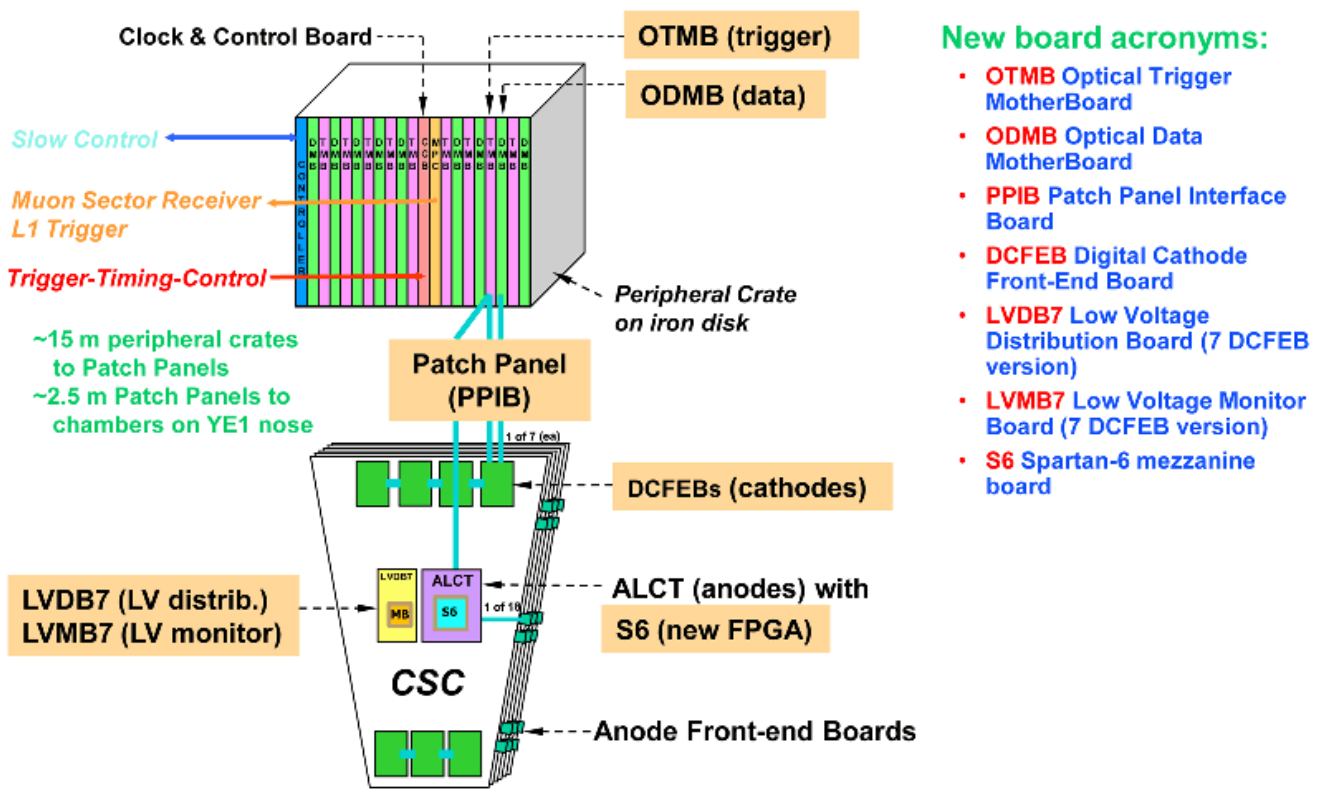
\includegraphics[width=0.90\linewidth]{figures/ME11_upgrade_overview.png}
                \caption{Schematic overview of the ME1/1 chambers upgrade.}
                \label{fig:me11_upgrade_overview}
        \end{center}
\end{figure}

\begin{figure}[htb]
        \begin{center}
                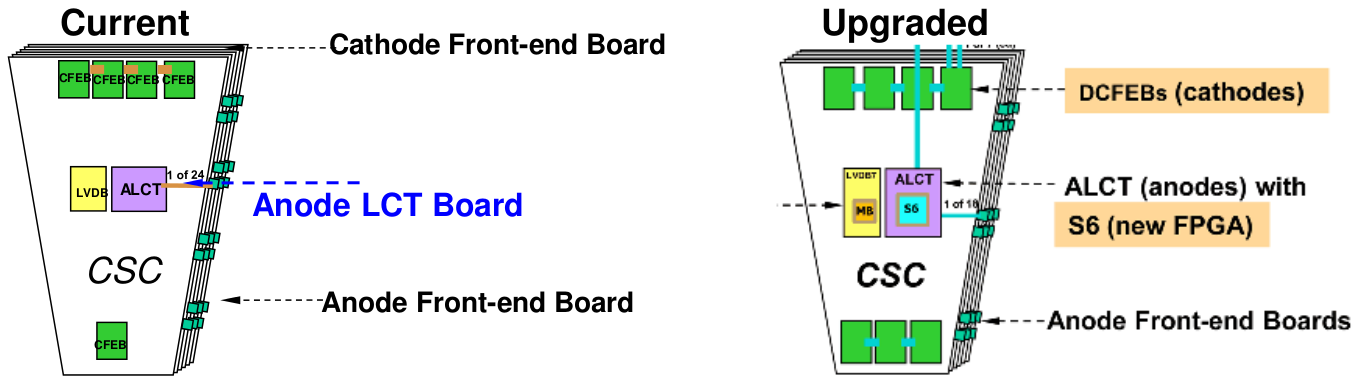
\includegraphics[width=0.90\linewidth]{figures/ME11_upgrade_electronics.png}
                \caption{Schematic overview of the ME1/1 electronics upgrade.}
                \label{fig:me11_upgrade_electronics}
        \end{center}
\end{figure}